%!TEX root = ../article.tex
\subsection{Cluster View}
% To enable users to observe the statistics of both the features and hidden states (\textbf{T1},\textbf{T2}), we develop the Cluster View (Fig.~\ref{fig:teaser}).
% It shows the overview of response relationship (\textbf{T3}) between the hidden units and features. The hidden units and features are visualized as the Hidden State Distribution and the Feature Glyph respectively.

The Cluster View (Fig.~\ref{fig:teaser}A) shows the overview of response relationship (\textbf{T3}) between the hidden units and features. The hidden units and features are visualized as the Hidden State Distribution and the Feature Glyph respectively.


\begin{figure}[t]
	\centering
    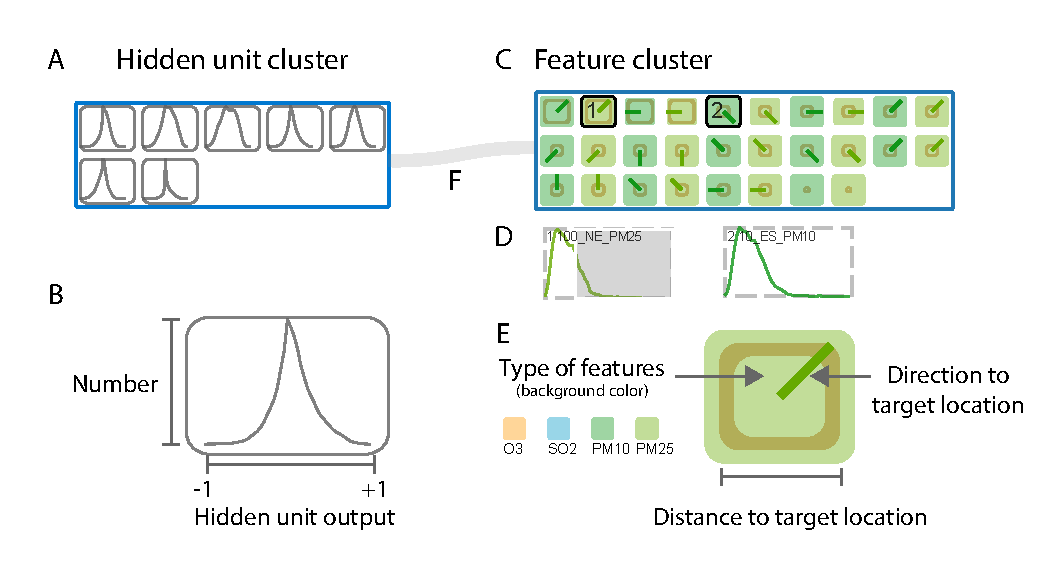
\includegraphics[width=0.45\textwidth]{pictures/design/cluster_design.pdf}
	\vspace{-3mm}
	\caption{Design of Hidden unit distribution and feature glyph. A) Hidden unit cluster; B) Hidden unit distribution; C) Feature cluster; D) Feature distribution for selected features; E) Feature glyph design; G) Response link}
	\label{fig:cluster_design}
	\vspace{-4mm}
\end{figure}


\textbf{Hidden State Distribution.}
The left column on the Cluster View is the Hidden State Distribution component.
As shown in Fig.~\ref{fig:cluster_design}A, each row represents a hidden unit cluster.
% The row height increases with the number of hidden states in each cluster.
Each hidden unit in a cluster is represented as a line chart that shows its activation distribution(\textbf{T1}).
The x-axis represents the hidden unit output ranging from $-1$ to $+1$ and the y-axis represents the \UC{corresponding probability} (Fig.~\ref{fig:cluster_design}B).
From the line chart, users can observe and compare the activation distribution patterns of different hidden units. 

\textbf{Feature Glyph.}
The right column of the Cluster View is the Feature Glyph component (Fig.~\ref{fig:cluster_design}C).
Similar to the Hidden State Distribution, each row represents a feature cluster in which a glyph (Fig.~\ref{fig:cluster_design}D) represents a feature.
As described in Sec.~\ref{section:application}, we define our usage scenario as air pollution forecasting.
Each feature has three identifiers: the feature category, the direction, and the distance from the feature to the target location.
The background color of the feature glyph cell encodes the feature category.
We use a categorical color scheme to encode different categories, and users can find the color legend at the top of the Cluster View.
\UC{In each feature glyph, the distance and direction to the target location are presented by a rectangle and a line segment with one end point at the center.}
The angle of the direction bar encodes the direction, and the width of the distance rectangle represents the distance(Fig.~\ref{fig:cluster_design}D).

\textbf{Interactions.}
We also support various interactions to allow users to dynamically explore this view.
The curves linking the hidden state cluster and feature cluster with the width indicate the response strength (Fig.~\ref{fig:cluster_design}E). Users can also filter the link according to the response strength by adjusting the slider bar. 
When hovering over a hidden state cluster or a feature cluster, the corresponding links and linked clusters will be highlighted.

In this view, the users can obtain an overview of the response relationship between hidden units and features, for example, we can find that there are not strong links connecting to cluster 8 (Fig.~\ref{fig:teaser} A$_3$), this may be because that all the hidden units are ``weakly'' activated in cluster 8.
% Users can also select a feature for further examination by clicking the corresponding feature cell.
% After clicking, a line chart will be appended to the right of the Feature Distribution component (Fig.~\ref{fig:cluster_design}D) to show the feature's value distribution.
